% Options for packages loaded elsewhere
\PassOptionsToPackage{unicode}{hyperref}
\PassOptionsToPackage{hyphens}{url}
%
\documentclass[
]{article}
\usepackage{amsmath,amssymb}
\usepackage{lmodern}
\usepackage{ifxetex,ifluatex}
\ifnum 0\ifxetex 1\fi\ifluatex 1\fi=0 % if pdftex
  \usepackage[T1]{fontenc}
  \usepackage[utf8]{inputenc}
  \usepackage{textcomp} % provide euro and other symbols
\else % if luatex or xetex
  \usepackage{unicode-math}
  \defaultfontfeatures{Scale=MatchLowercase}
  \defaultfontfeatures[\rmfamily]{Ligatures=TeX,Scale=1}
  \setmainfont[]{serif}
\fi
% Use upquote if available, for straight quotes in verbatim environments
\IfFileExists{upquote.sty}{\usepackage{upquote}}{}
\IfFileExists{microtype.sty}{% use microtype if available
  \usepackage[]{microtype}
  \UseMicrotypeSet[protrusion]{basicmath} % disable protrusion for tt fonts
}{}
\makeatletter
\@ifundefined{KOMAClassName}{% if non-KOMA class
  \IfFileExists{parskip.sty}{%
    \usepackage{parskip}
  }{% else
    \setlength{\parindent}{0pt}
    \setlength{\parskip}{6pt plus 2pt minus 1pt}}
}{% if KOMA class
  \KOMAoptions{parskip=half}}
\makeatother
\usepackage{xcolor}
\IfFileExists{xurl.sty}{\usepackage{xurl}}{} % add URL line breaks if available
\IfFileExists{bookmark.sty}{\usepackage{bookmark}}{\usepackage{hyperref}}
\hypersetup{
  pdftitle={Spatiotemporal Impacts of Ideology and Social Vulnerability on COVID-19: Supplemental Appendix},
  pdfauthor={Erich Seamon, Jennifer-Johnson Leung, Craig Miller, Ben Ridenhour},
  hidelinks,
  pdfcreator={LaTeX via pandoc}}
\urlstyle{same} % disable monospaced font for URLs
\usepackage[margin=1in]{geometry}
\usepackage{graphicx}
\makeatletter
\def\maxwidth{\ifdim\Gin@nat@width>\linewidth\linewidth\else\Gin@nat@width\fi}
\def\maxheight{\ifdim\Gin@nat@height>\textheight\textheight\else\Gin@nat@height\fi}
\makeatother
% Scale images if necessary, so that they will not overflow the page
% margins by default, and it is still possible to overwrite the defaults
% using explicit options in \includegraphics[width, height, ...]{}
\setkeys{Gin}{width=\maxwidth,height=\maxheight,keepaspectratio}
% Set default figure placement to htbp
\makeatletter
\def\fps@figure{htbp}
\makeatother
\setlength{\emergencystretch}{3em} % prevent overfull lines
\providecommand{\tightlist}{%
  \setlength{\itemsep}{0pt}\setlength{\parskip}{0pt}}
\setcounter{secnumdepth}{-\maxdimen} % remove section numbering
\usepackage[export]{adjustbox}
\usepackage{booktabs}
\usepackage{longtable}
\usepackage{array}
\usepackage{multirow}
\usepackage{wrapfig}
\usepackage{float}
\usepackage{colortbl}
\usepackage{pdflscape}
\usepackage{tabu}
\usepackage{threeparttable}
\usepackage{threeparttablex}
\usepackage[normalem]{ulem}
\usepackage{makecell}
\usepackage{xcolor}
\ifluatex
  \usepackage{selnolig}  % disable illegal ligatures
\fi

\title{Spatiotemporal Impacts of Ideology and Social Vulnerability on
COVID-19: Supplemental Appendix}
\author{Erich Seamon, Jennifer-Johnson Leung, Craig Miller, Ben
Ridenhour}
\date{01/30/2023}

\begin{document}
\maketitle

{
\setcounter{tocdepth}{2}
\tableofcontents
}
\newpage

\hypertarget{appendix-overview}{%
\section{Appendix Overview}\label{appendix-overview}}

\hypertarget{summary}{%
\subsection{Summary}\label{summary}}

Below are examinations of COVID-19 cumulative deaths adjusted by
population, at a county level. We look at spatial and temporal
variations for the entire United States, as well by region.

\hypertarget{part-1-study-area-and-regionalization}{%
\subsection{Part 1: Study Area and
Regionalization}\label{part-1-study-area-and-regionalization}}

Regionalization is based on United States(US) Health and Human Services
(HHS) health regions.

\begin{itemize}
\tightlist
\item
  Region 1 and 2 (combined): NorthEast: Connecticut, Maine,
  Massachusetts, New Hampshire, Rhode Island, Vermont, New York and New
  Jersey
\item
  Region 3: MidEast: Pennsylvania, West Virginia, Maryland, Delaware,
  Virginia and the District of Columbia
\item
  Region 4: SouthEast: Florida, Georgia, South Carolina, and North
  Carolina, Alabama, Mississippi, Tennessee, and Kentucky
\item
  Region 5: Midwest: Ohio, Indiana, Illinois, Michigan, Wisconsin, and
  Minnesota
\item
  Region 6: MidSouth: Texas, Louisiana, Arkansas, and New Mexico,
  Oklahoma
\item
  Region 7: Middle West: Iowa, Missouri, Nebraska, and Kansas
\item
  Region 8: MidNorth: Montana, Wyoming, Utah, Colorado, North Dakota,
  and South Dakota
\item
  Region 9: West: California, Nevada, and Arizona
\item
  Region 10: Pacific Northwest: Idaho, Oregon, and Washington
\end{itemize}

\hypertarget{part-2-datasets-and-modeling-framework}{%
\subsection{Part 2: Datasets and Modeling
Framework}\label{part-2-datasets-and-modeling-framework}}

Part 2 of our analysis documents the datasets and modeling methodology
employed as part of this effort.

\hypertarget{part-3-exploratory-data-analysis-and-regression-modeling}{%
\subsection{Part 3: Exploratory Data Analysis and Regression
Modeling}\label{part-3-exploratory-data-analysis-and-regression-modeling}}

Our regional analysis examines COVID-19 parameters for the entire United
States, as well as for each of the nine (9) regions listed above.

\begin{itemize}
\item
  The first plot (1) shows fatality rates vs.~logarithmic population
  density, categorized by voting ideology summarized by the 2020
  Presidential Election. 100-75\% vote for Biden = very liberal, 75-50\%
  for Biden = moderately liberal, 100-75\% for Trump = very
  conservative, and 75-50\% for Trump = moderately conservative. Each
  observation represents one county.
\item
  The second plot (2) shows cumulative cases, adjusted for population,
  vs.~cumulative deaths, adjusted for population, categorized by voting
  ideology - as noted above.
\item
  The third (3) and fourth (4) plots show the relationship of the four
  ideology groupings across the specified region, over time - examining
  deaths for a rolling window, as well as cumulative deaths. These plots
  provide a summary view of the change in ideological and regional
  associations with cases and deaths.
\end{itemize}

For each region, we have outputs for three linear linear models, with
population adjusted deaths (by county) as the dependent variable - for
each of the three time windows (alpha, delta, and omicron variant). In
addition, we have standardized coefficients graphs, that indicates the
effect for each variable, for each model.

\newpage

\hypertarget{part-4-spatial-autocorrelation}{%
\subsection{Part 4: Spatial
Autocorrelation}\label{part-4-spatial-autocorrelation}}

The second portion of this analysis evaluates the spatial
autocorrelation of population adjusted county deaths, for all three time
periods examined.

\hypertarget{part-5-geographically-weighted-random-forest-gwrf-modeling}{%
\subsection{Part 5: Geographically Weighted Random Forest (GWRF)
Modeling}\label{part-5-geographically-weighted-random-forest-gwrf-modeling}}

The third portion of this analysis attempts to model spatial variation
for the entire United States, using geographically weighted random
forest modeling (GWRF). Our model incorporates the same independent
variables that are used as part of our regionalized linear models.

Geographical Weighted Random Forest (GWRF) is a spatial analysis method
using a local version of the Random Forest Regression Model. It allows
for the investigation of spatial non-stationarity, and the relationship
between a dependent and a set of independent variables. The latter is
possible by fitting a sub-model for each observation in space, taking
into account the neighboring observations. This technique adopts the
idea of the Geographically Weighted Regression Kalogirou (2003). The
main difference between a tradition (linear) GWR and GRF is that we can
model non-stationarity coupled with a flexible non-linear model which is
very hard to overfit due to its bootstrapping nature, thus relaxing the
assumptions of traditional Gaussian statistics. Essentially it was
designed to be a bridge between machine learning and geographical
models, combining inferential and explanatory power. Additionally, it is
suited for datasets with numerous predictors, due to the robust nature
of the random forest algorithm with regards to high dimensionality.

For this analysis, We generate GWRF localized model fits and feature
importances (IncMSE). The feature importance algorithmic process is:

\begin{enumerate}
\def\labelenumi{\arabic{enumi}.}
\tightlist
\item
  Compute model MSE
\item
  For each variable in the model:

  \begin{enumerate}
  \def\labelenumii{\alph{enumii}.}
  \tightlist
  \item
    Permute variable
  \item
    Calculate new model MSE according to variable permutation
  \item
    Take the difference between model MSE and new model MSE
  \end{enumerate}
\item
  Collect the results in a list
\end{enumerate}

\newpage

\hypertarget{part-1-study-area-and-regionalization-1}{%
\section{Part 1: Study Area and
Regionalization}\label{part-1-study-area-and-regionalization-1}}

For the initial portion of our analysis, we examine COVID-19 cases and
deaths for the entire United States, as well as by U.S. Human Health
Services (HHS) regions, as noted in Figure S1 below.

\hypertarget{figure-s1-study-area}{%
\subsection{Figure S1: Study Area}\label{figure-s1-study-area}}

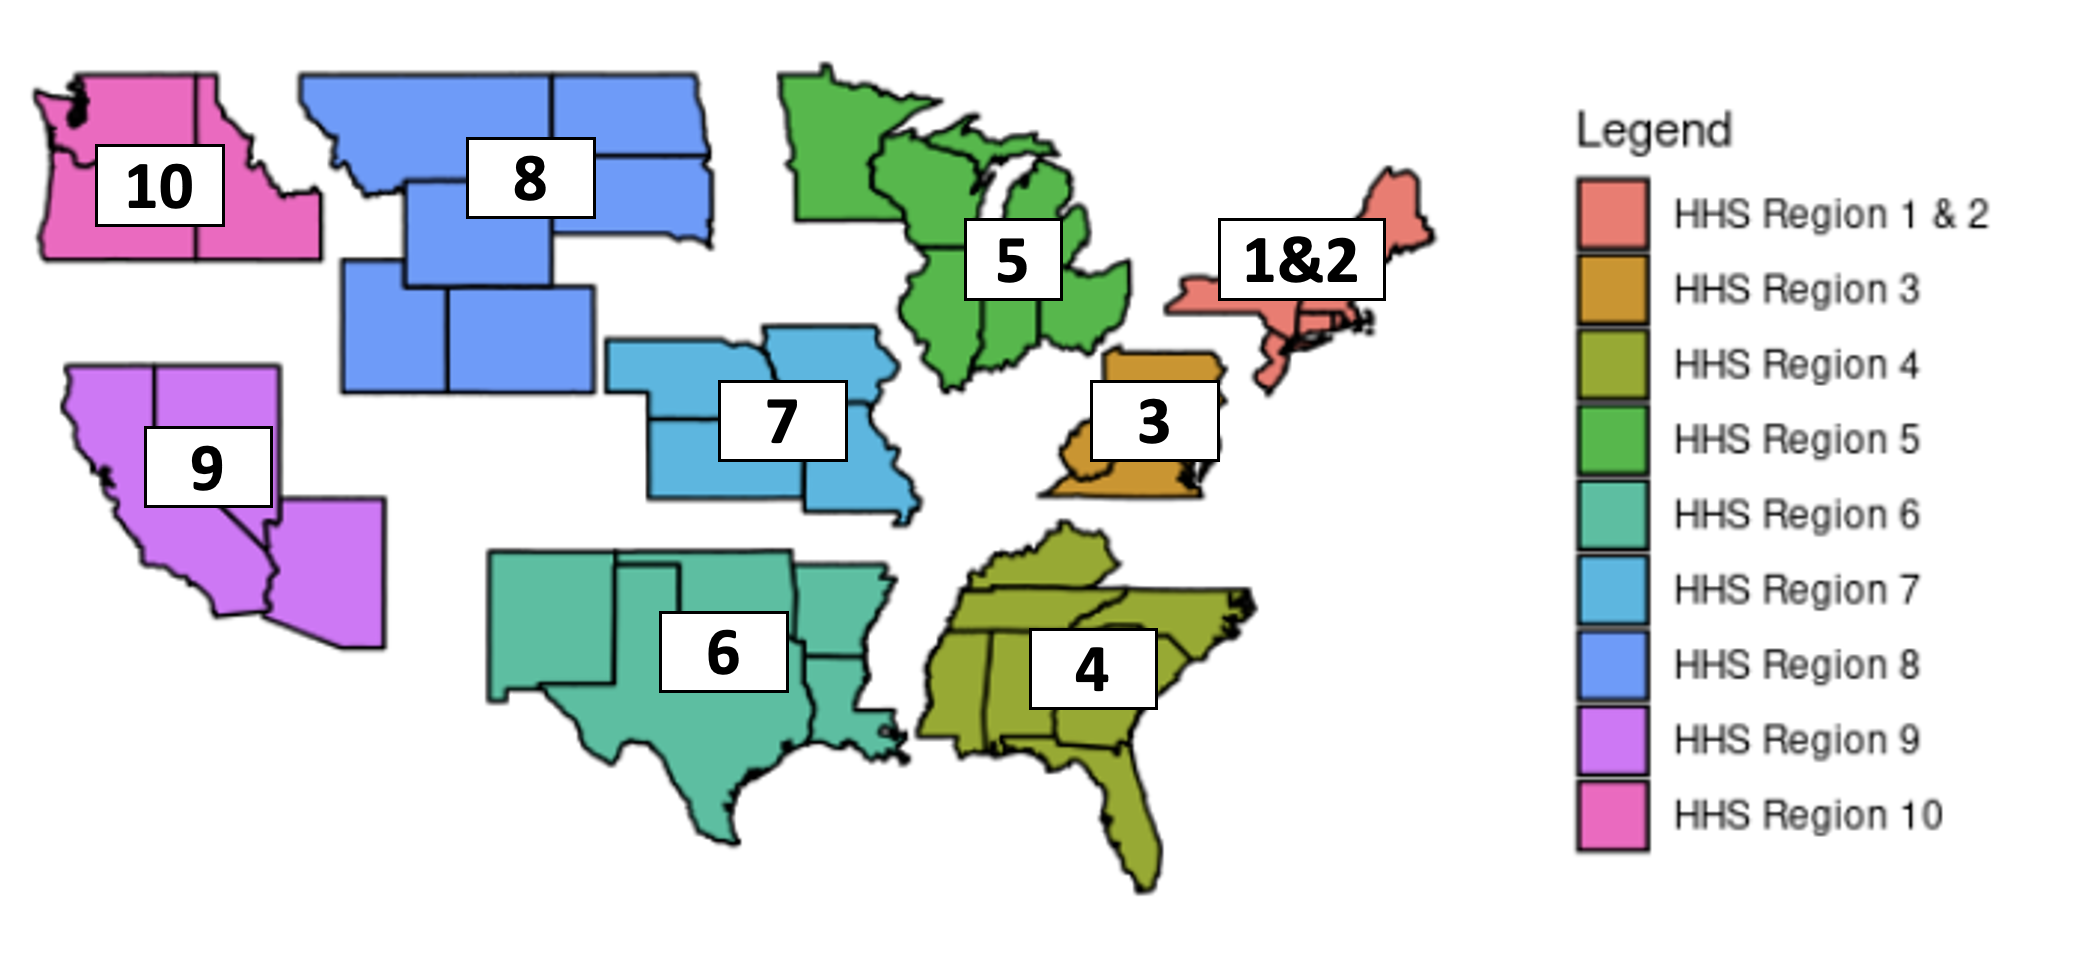
\includegraphics[width=1\textwidth,height=1\textheight]{../figures/hhs_regions.png}

\newpage

\hypertarget{part-2-datasets-and-modeling-framework-1}{%
\section{Part 2: Datasets and Modeling
Framework}\label{part-2-datasets-and-modeling-framework-1}}

We utilize fifteen (15) independent variables and one (1) dependent
variable for our analysis, which are as follows:

\hypertarget{table-t1-variable-descriptions}{%
\subsection{Table T1: Variable
Descriptions}\label{table-t1-variable-descriptions}}

\begin{table}[!h]

\caption{\label{tab:unnamed-chunk-3}Table T1: Variable Descriptions. * = dependent variable}
\centering
\resizebox{\linewidth}{!}{
\fontsize{10}{12}\selectfont
\begin{tabular}[t]{>{\raggedright\arraybackslash}p{2in}|>{\raggedright\arraybackslash}p{2in}|>{\raggedright\arraybackslash}p{3in}}
\hline
Variables & Description & Data Source\\
\hline
Socioeconomic Status & Index which represents income, poverty, employment, and education. & \\
\cline{1-2}
Household Composition and Disability & Index with represents age, single parenting, and disability. & \\
\cline{1-2}
Minority Status & Index which represents race and ethnicity. & \\
\cline{1-2}
Housing Type and Transportation & Index which represents housing structure, crowding and vehicle access. & \multirow{-4}{3in}{\raggedright\arraybackslash Social Vulnerability Indices (SVI) taken from the US Census agency for toxic substances and disease registry (ATSDR)}\\
\cline{1-3}
Obesity & Number of people who are obese, at a county level. & \\
\cline{1-2}
Unemployment & Number of unemployed adults per county. & \\
\cline{1-2}
Uninsured Adults & Number of uninsured adults per county. & \\
\cline{1-2}
Social Associations & Number of people who are members of a social organization (churches, clubs, etc). & \\
\cline{1-2}
Diabetes & Number of people with diabetes at a county level. & \\
\cline{1-2}
Food Insecurity & Index indicating the relative level of food insecurity in a county. & \\
\cline{1-2}
Broadband Access & Number of people without broadband access. & \multirow{-7}{3in}{\raggedright\arraybackslash University of Wisconsin's Population Health Institute}\\
\cline{1-3}
Population Density & Population density at a county level. & \\
\cline{1-2}
Population Age 65+ & Number of people age 65 or older in a county. & \multirow{-2}{3in}{\raggedright\arraybackslash 2020 US Census}\\
\cline{1-3}
Democratic Voting Percentage & Represents voting outcomes from the 2020 presidential general election. & Massachusettes Institute of Technology's (MIT) Election Lab\\
\cline{1-3}
Vaccination Rate & CDC data for two dose vaccination rates at a county level, ending in April 1, 2022. & \\
\cline{1-2}
Population adjusted COVID-19 deaths* & Population-adjusted COVID-19 deaths per county. & \multirow{-2}{3in}{\raggedright\arraybackslash US Centers for Disease Control (CDC)}\\
\hline
\end{tabular}}
\end{table}

Using this framework, we constructed three (3) temporal model time
frames:

\begin{enumerate}
\def\labelenumi{\arabic{enumi}.}
\tightlist
\item
  Alpha variant time window (deaths calculated from December 1, 2019 to
  May 1, 2021)
\item
  Delta variant time window (deaths calculated from May 1, 2021, to
  December 1, 2021)
\item
  Omicron variant time window (deaths calculated from December 1, 2021
  to April 1, 2022)
\end{enumerate}

\newpage

\hypertarget{figure-s2-model-framework}{%
\subsection{Figure S2: Model
Framework}\label{figure-s2-model-framework}}

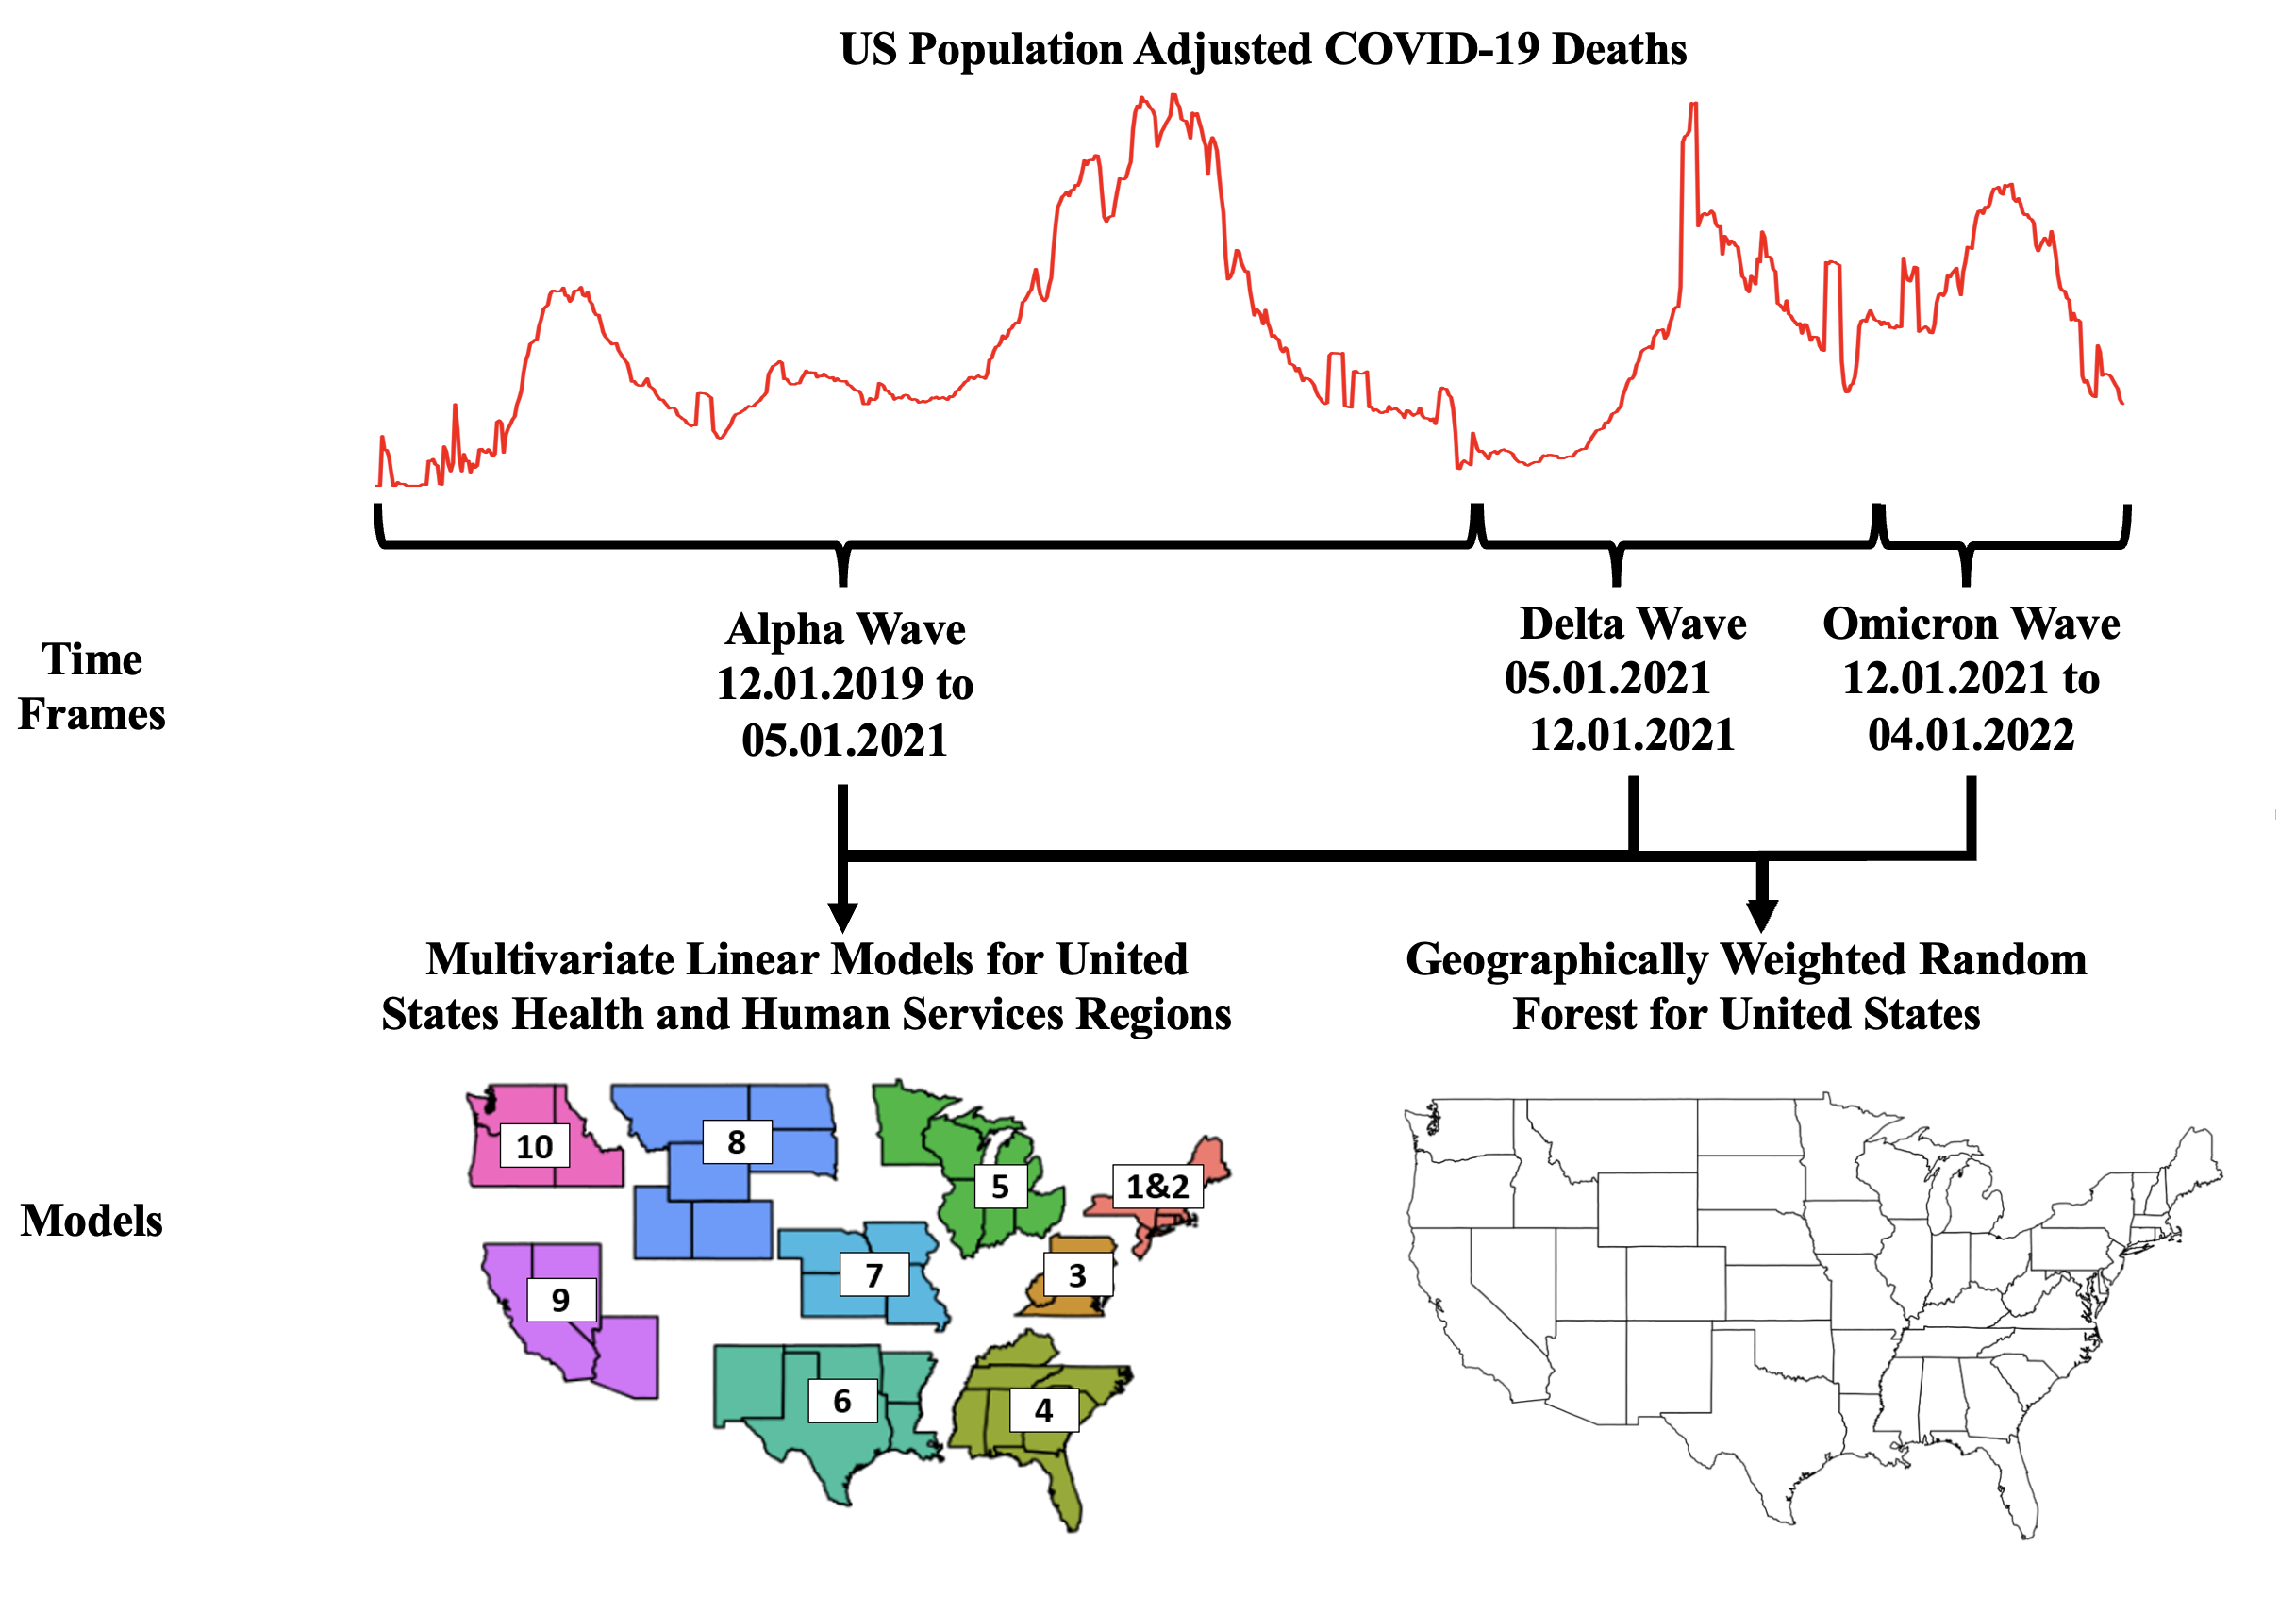
\includegraphics[width=1\textwidth,height=1\textheight]{../figures/model.png}

\newpage

\hypertarget{figure-s3-dataset-visualizations}{%
\subsection{Figure S3: Dataset
Visualizations}\label{figure-s3-dataset-visualizations}}

\includegraphics{test_0426_files/figure-latex/datapanel2-1.pdf}

\includegraphics{test_0426_files/figure-latex/datapanel3-1.pdf}

\includegraphics{test_0426_files/figure-latex/datapanel4-1.pdf}
\includegraphics{test_0426_files/figure-latex/datapanel4-2.pdf}

\newpage

\includegraphics{test_0426_files/figure-latex/datapanel5-1.pdf}

\newpage

\hypertarget{figure-s4-correlation-heatmap}{%
\subsection{Figure S4: Correlation
HeatMap}\label{figure-s4-correlation-heatmap}}

\includegraphics{test_0426_files/figure-latex/unnamed-chunk-4-1.pdf}

\newpage

\hypertarget{part-3-data-analysis-and-regression-united-states}{%
\section{Part 3: Data Analysis and Regression: United
States}\label{part-3-data-analysis-and-regression-united-states}}

\hypertarget{figure-s5-fatality-rate-vs.-population-density}{%
\subsection{Figure S5: Fatality Rate vs.~Population
Density}\label{figure-s5-fatality-rate-vs.-population-density}}

\includegraphics{test_0426_files/figure-latex/unnamed-chunk-6-1.pdf}

\hypertarget{figure-s6-county-level-cumulative-cases-vs.-cumulative-deaths}{%
\subsection{Figure S6: County Level Cumulative Cases vs.~Cumulative
Deaths}\label{figure-s6-county-level-cumulative-cases-vs.-cumulative-deaths}}

\includegraphics{test_0426_files/figure-latex/unnamed-chunk-7-1.pdf}

\hypertarget{figure-s7-population-adjusted-cumulative-deaths-vs-ideology-over-time}{%
\subsection{Figure S7: Population Adjusted Cumulative Deaths vs Ideology
over
time}\label{figure-s7-population-adjusted-cumulative-deaths-vs-ideology-over-time}}

\includegraphics{test_0426_files/figure-latex/unnamed-chunk-16-1.pdf}

\hypertarget{table-t2-united-states-regression-model-results}{%
\subsection{Table T2: United States: Regression Model
Results}\label{table-t2-united-states-regression-model-results}}

\begin{table}
\centering
\begin{tabular}{lrlrlrl}
\toprule
\multicolumn{1}{c}{ } & \multicolumn{2}{c}{Alpha Wave} & \multicolumn{2}{c}{Delta Wave} & \multicolumn{2}{c}{Omicron Wave} \\
\cmidrule(l{3pt}r{3pt}){2-3} \cmidrule(l{3pt}r{3pt}){4-5} \cmidrule(l{3pt}r{3pt}){6-7}
  & Estimates & Adjusted P values & Estimates & Adjusted P values & Estimates & Adjusted P values\\
\midrule
Intercept & -7.73313 & \textbf{0} & -7.05210 & \textbf{0} & -7.49889 & \textbf{0}\\
Socioeconomic & 0.04435 & 1 & -0.03913 & 1 & 0.05413 & 1\\
Household Composition & Disability & 0.26958 & \textbf{2.84e-07} & 0.28751 & \textbf{3.83e-09} & 0.36952 & \textbf{1.7e-14}\\
Housing Type & Transportation & 0.11719 & 0.57 & 0.20256 & \textbf{5.18e-05} & -0.09546 & 1\\
Unemployed & 0.86481 & \textbf{5.59e-13} & -0.06978 & 1 & 0.33055 & 1\\
\addlinespace
Food Insecurity & -1.22957 & \textbf{6.24e-47} & 1.02947 & \textbf{1.21e-31} & 0.04276 & 1\\
Broadband Access & 2.87818 & \textbf{2.49e-60} & -0.99263 & \textbf{3.65e-06} & 1.17898 & \textbf{2.31e-08}\\
Diabetes & 0.71078 & \textbf{2.65e-13} & 1.30850 & \textbf{4.96e-48} & 0.49088 & \textbf{1.89e-05}\\
Obesity & -0.22955 & 1 & -0.49613 & \textbf{2.47e-06} & 0.27717 & 0.381\\
Population Density & 0.09549 & \textbf{6.62e-42} & -0.01686 & 1 & 0.05980 & \textbf{8.87e-14}\\
\addlinespace
Associations & 1.46995 & \textbf{2.52e-18} & -0.94949 & \textbf{6.9e-07} & 0.23206 & 1\\
Age over 65 & 0.00000 & \textbf{1.03e-18} & 0.00000 & 1 & 0.00000 & \textbf{7.46e-13}\\
Democratic Voting Pct & -0.62271 & \textbf{1.3e-11} & -1.41023 & \textbf{1.77e-59} & -0.98851 & \textbf{5.87e-27}\\
Vaccination Rate & -0.08105 & 1 & -0.29546 & 1 & -0.35674 & 0.368\\
Minority Status and Language & 0.44996 & \textbf{1.88e-19} & -0.32104 & \textbf{4.78e-10} & -0.24493 & \textbf{4.06e-05}\\
\addlinespace
Uninsured Adults & -0.10371 & 1 & 1.25487 & \textbf{3.2e-89} & -0.56820 & \textbf{1.15e-15}\\
\bottomrule
\multicolumn{7}{l}{\rule{0pt}{1em}\textit{Note: }}\\
\multicolumn{7}{l}{\rule{0pt}{1em}Bold = significant value}\\
\end{tabular}
\end{table}

\begin{table}
\centering
\begin{tabular}{lrrr}
\toprule
  & Alpha Wave & Delta Wave & Omicron Wave\\
\midrule
Pseudo R2 & 0.416 & 0.675 & 0.505\\
\bottomrule
\end{tabular}
\end{table}

\newpage

\newpage

\hypertarget{part-3-data-analysis-and-regression-regions-1-and-2-northeast}{%
\section{Part 3: Data Analysis and Regression: Regions 1 and 2
(Northeast)}\label{part-3-data-analysis-and-regression-regions-1-and-2-northeast}}

\hypertarget{figure-s8-population-adjusted-cumulative-deaths-vs-ideology-over-time}{%
\subsection{Figure S8: Population Adjusted Cumulative Deaths vs Ideology
over
time}\label{figure-s8-population-adjusted-cumulative-deaths-vs-ideology-over-time}}

\includegraphics{test_0426_files/figure-latex/unnamed-chunk-37-1.pdf}

\hypertarget{table-t3-region-1-2-northeast-regression-model-results}{%
\subsection{Table T3: Region 1 \& 2 (Northeast): Regression Model
Results}\label{table-t3-region-1-2-northeast-regression-model-results}}

\includegraphics{test_0426_files/figure-latex/unnamed-chunk-41-1.png}

\newpage

\hypertarget{part-3-data-analysis-and-regression-region-3-mideast}{%
\section{Part 3: Data Analysis and Regression: Region 3
(Mideast)}\label{part-3-data-analysis-and-regression-region-3-mideast}}

\hypertarget{figure-s9-population-adjusted-cumulative-deaths-vs-ideology-over-time}{%
\subsection{Figure S9: Population Adjusted Cumulative Deaths vs Ideology
over
time}\label{figure-s9-population-adjusted-cumulative-deaths-vs-ideology-over-time}}

\includegraphics{test_0426_files/figure-latex/unnamed-chunk-53-1.pdf}

\hypertarget{table-t4-region-3-mideast-regression-model-results}{%
\subsection{Table T4: Region 3 (Mideast): Regression Model
Results}\label{table-t4-region-3-mideast-regression-model-results}}

\includegraphics{test_0426_files/figure-latex/unnamed-chunk-57-1.png}

\newpage

\hypertarget{part-3-data-analysis-and-regression-region-4-southeast}{%
\section{Part 3: Data Analysis and Regression: Region 4
(Southeast)}\label{part-3-data-analysis-and-regression-region-4-southeast}}

\hypertarget{figure-s10-population-adjusted-cumulative-deaths-vs-ideology-over-time}{%
\subsection{Figure S10: Population Adjusted Cumulative Deaths vs
Ideology over
time}\label{figure-s10-population-adjusted-cumulative-deaths-vs-ideology-over-time}}

\includegraphics{test_0426_files/figure-latex/unnamed-chunk-69-1.pdf}

\hypertarget{table-t5-region-4-southeast-regression-model-results}{%
\subsection{Table T5: Region 4 (Southeast): Regression Model
Results}\label{table-t5-region-4-southeast-regression-model-results}}

\includegraphics{test_0426_files/figure-latex/unnamed-chunk-73-1.png}

\newpage

\hypertarget{part-3-data-analysis-and-regression-region-5-midwest}{%
\section{Part 3: Data Analysis and Regression: Region 5
(Midwest)}\label{part-3-data-analysis-and-regression-region-5-midwest}}

\hypertarget{figure-s11-population-adjusted-cumulative-deaths-vs-ideology-over-time}{%
\subsection{Figure S11: Population Adjusted Cumulative Deaths vs
Ideology over
time}\label{figure-s11-population-adjusted-cumulative-deaths-vs-ideology-over-time}}

\includegraphics{test_0426_files/figure-latex/unnamed-chunk-85-1.pdf}

\hypertarget{table-t6-region-5-midwest-regression-model-results}{%
\subsection{Table T6: Region 5 (Midwest): Regression Model
Results}\label{table-t6-region-5-midwest-regression-model-results}}

\includegraphics{test_0426_files/figure-latex/unnamed-chunk-89-1.png}

\newpage

\hypertarget{part-3-data-analysis-and-regression-region-6-midsouth}{%
\section{Part 3: Data Analysis and Regression: Region 6
(MidSouth)}\label{part-3-data-analysis-and-regression-region-6-midsouth}}

\hypertarget{figure-s12-population-adjusted-cumulative-deaths-vs-ideology-over-time}{%
\subsection{Figure S12: Population Adjusted Cumulative Deaths vs
Ideology over
time}\label{figure-s12-population-adjusted-cumulative-deaths-vs-ideology-over-time}}

\includegraphics{test_0426_files/figure-latex/unnamed-chunk-101-1.pdf}

\hypertarget{table-t7-region-6-midsouth-regression-model-results}{%
\subsection{Table T7: Region 6 (Midsouth): Regression Model
Results}\label{table-t7-region-6-midsouth-regression-model-results}}

\includegraphics{test_0426_files/figure-latex/unnamed-chunk-105-1.png}

\newpage

\hypertarget{part-3-data-analysis-and-regression-region-7-middle-west}{%
\section{Part 3: Data Analysis and Regression: Region 7 (Middle
West)}\label{part-3-data-analysis-and-regression-region-7-middle-west}}

\hypertarget{figure-s13-population-adjusted-cumulative-deaths-vs-ideology-over-time}{%
\subsection{Figure S13: Population Adjusted Cumulative Deaths vs
Ideology over
time}\label{figure-s13-population-adjusted-cumulative-deaths-vs-ideology-over-time}}

\includegraphics{test_0426_files/figure-latex/unnamed-chunk-117-1.pdf}

\hypertarget{table-t8-region-7-middle-west-regression-model-results}{%
\subsection{Table T8: Region 7 (Middle West): Regression Model
Results}\label{table-t8-region-7-middle-west-regression-model-results}}

\includegraphics{test_0426_files/figure-latex/unnamed-chunk-121-1.png}

\newpage

\hypertarget{part-3-data-analysis-and-regression-region-8-midnorth}{%
\section{Part 3: Data Analysis and Regression: Region 8
(Midnorth)}\label{part-3-data-analysis-and-regression-region-8-midnorth}}

\hypertarget{figure-s14-population-adjusted-cumulative-deaths-vs-ideology-over-time}{%
\subsection{Figure S14: Population Adjusted Cumulative Deaths vs
Ideology over
time}\label{figure-s14-population-adjusted-cumulative-deaths-vs-ideology-over-time}}

\includegraphics{test_0426_files/figure-latex/unnamed-chunk-133-1.pdf}

\hypertarget{table-t9-region-8-midnorth-regression-model-results}{%
\subsection{Table T9: Region 8 (Midnorth): Regression Model
Results}\label{table-t9-region-8-midnorth-regression-model-results}}

\includegraphics{test_0426_files/figure-latex/unnamed-chunk-137-1.png}

\newpage

\hypertarget{part-3-data-analysis-and-regression-region-9-west}{%
\section{Part 3: Data Analysis and Regression: Region 9
(West)}\label{part-3-data-analysis-and-regression-region-9-west}}

\hypertarget{figure-s15-population-adjusted-cumulative-deaths-vs-ideology-over-time}{%
\subsection{Figure S15: Population Adjusted Cumulative Deaths vs
Ideology over
time}\label{figure-s15-population-adjusted-cumulative-deaths-vs-ideology-over-time}}

\includegraphics{test_0426_files/figure-latex/unnamed-chunk-149-1.pdf}

\hypertarget{table-t10-region-9-west-regression-model-results}{%
\subsection{Table T10: Region 9 (West): Regression Model
Results}\label{table-t10-region-9-west-regression-model-results}}

\includegraphics{test_0426_files/figure-latex/unnamed-chunk-153-1.png}

\newpage

\hypertarget{part-3-data-analysis-and-regression-region-10-pacific-nw}{%
\section{Part 3: Data Analysis and Regression: Region 10 (Pacific
NW)}\label{part-3-data-analysis-and-regression-region-10-pacific-nw}}

\hypertarget{figure-s16-population-adjusted-cumulative-deaths-vs-ideology-over-time}{%
\subsection{Figure S16: Population Adjusted Cumulative Deaths vs
Ideology over
time}\label{figure-s16-population-adjusted-cumulative-deaths-vs-ideology-over-time}}

\includegraphics{test_0426_files/figure-latex/unnamed-chunk-165-1.pdf}

\hypertarget{table-t11-region-10-pacific-northwest-regression-model-results}{%
\subsection{Table T11: Region 10 (Pacific Northwest): Regression Model
Results}\label{table-t11-region-10-pacific-northwest-regression-model-results}}

\includegraphics{test_0426_files/figure-latex/unnamed-chunk-169-1.png}

\newpage

\newpage

\hypertarget{part-3-data-analysis-and-regression-modeling-summarized-model-results}{%
\section{Part 3: Data Analysis and Regression Modeling Summarized Model
Results}\label{part-3-data-analysis-and-regression-modeling-summarized-model-results}}

\hypertarget{table-t12-model-results-alpha-wave-december-2019---may-2021}{%
\subsection{Table T12: Model Results: Alpha Wave (December 2019 - May
2021)}\label{table-t12-model-results-alpha-wave-december-2019---may-2021}}

\includegraphics{test_0426_files/figure-latex/unnamed-chunk-171-1.png}

\hypertarget{table-t13-model-results-delta-wave-may-2021---december-2021}{%
\subsection{Table T13: Model Results: Delta Wave (May 2021 - December
2021)}\label{table-t13-model-results-delta-wave-may-2021---december-2021}}

\includegraphics{test_0426_files/figure-latex/unnamed-chunk-172-1.png}

\hypertarget{table-t14-model-results-omicron-wave-december-2021---april-2022}{%
\subsection{Table T14: Model Results: Omicron Wave (December 2021 -
April
2022)}\label{table-t14-model-results-omicron-wave-december-2021---april-2022}}

\includegraphics{test_0426_files/figure-latex/unnamed-chunk-173-1.png}

\newpage

\hypertarget{table-t15-regionalized-regression-model-results-significance-table}{%
\subsection{Table T15: Regionalized Regression Model Results:
Significance
Table}\label{table-t15-regionalized-regression-model-results-significance-table}}

\begin{table}[!h]
\centering\begingroup\fontsize{8}{10}\selectfont

\begin{tabular}{l>{\raggedright\arraybackslash}p{1in}>{\raggedright\arraybackslash}p{.5in}>{\raggedright\arraybackslash}p{1in}>{\raggedright\arraybackslash}p{.5in}>{\raggedright\arraybackslash}p{1in}>{\raggedright\arraybackslash}p{.5in}>{\raggedright\arraybackslash}p{.5in}}
\toprule
Regions & Alpha & AlphaR2 & Delta & DeltaR2 & Omicron & OmicronR2 & Map\\
\midrule
Regions 1-2 & Household Composition, Unemployment, Food Insecurity, Broadband Access, Diabetes, Population Density, Social Associations, Age over 65+, Voting, Minority Status & 129 & Population Density, Voting & 129 & Vaccination Rate & 129 & 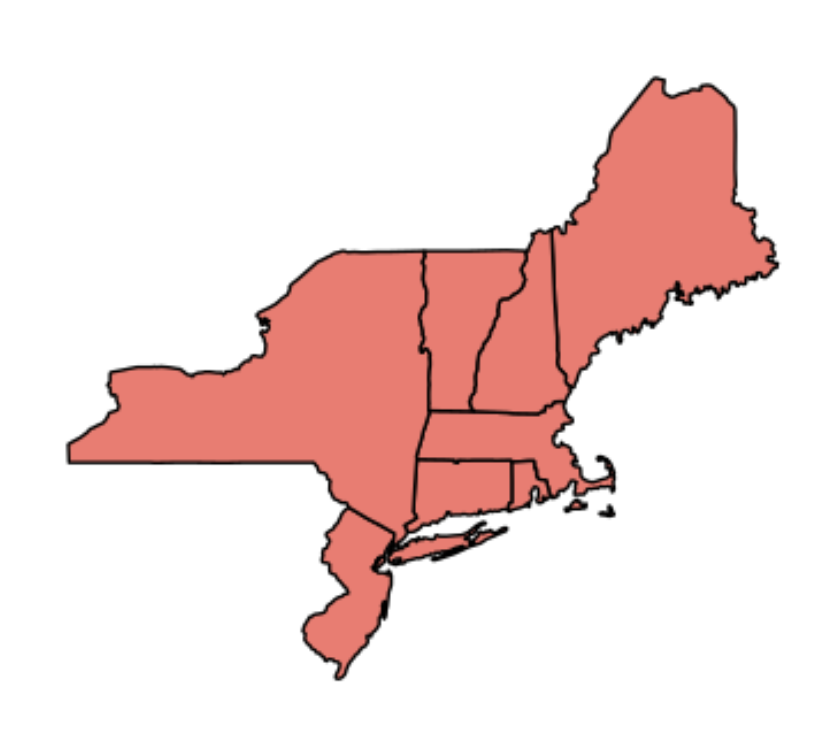
\includegraphics[valign = T,width=2cm]{/mnt/ceph/erichs/git/IMCI-covid-riskfinal/region_pngs/region1.png}\\
Region 3 & Food Insecurity, Social Associations & 89 & Broadband Access, Population Density, Voting, Minority Status & 87 & Socioeconomics, Household Composition, Uninsured Adults & 84 & 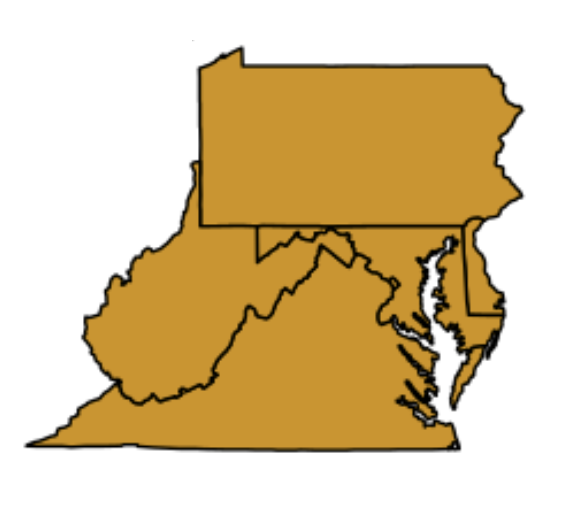
\includegraphics[valign = T,width=2cm]{/mnt/ceph/erichs/git/IMCI-covid-riskfinal/region_pngs/region3.png}\\
Region 4 & Socioeconomics, Food Insecurity, Social Associations, Age over 65+, Uninsured Adults & 291 & Household Composition, Housing Type, Voting, Vaccination Rate, Uninsured Adults & 291 & Diabetes, Vaccination Rate & 291 & 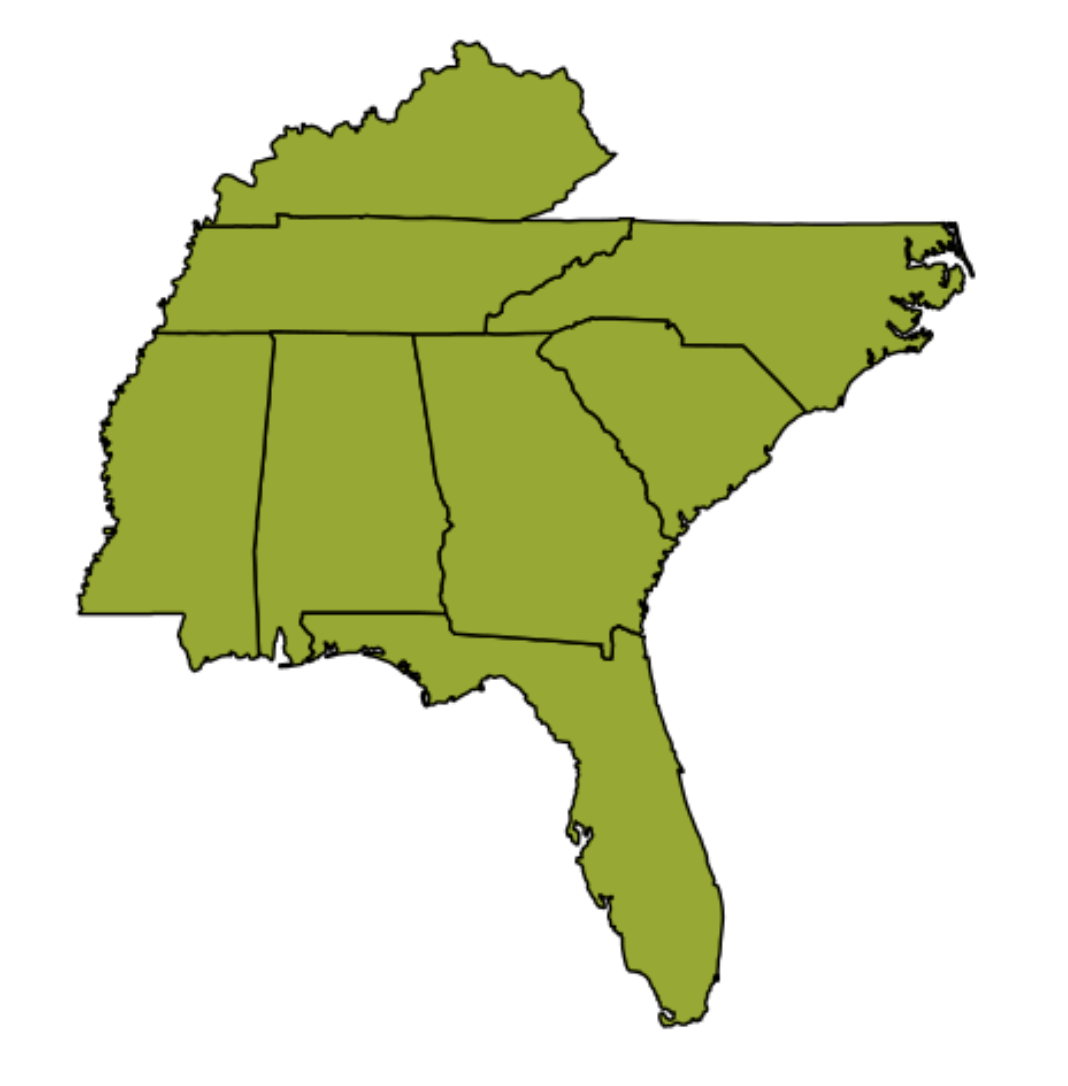
\includegraphics[valign = T,width=2cm]{/mnt/ceph/erichs/git/IMCI-covid-riskfinal/region_pngs/region4.png}\\
Region 5 & Socioeconomics, Household Composition, Broadband Access, Age over 65+, Uninsured Adults & 408 & Diabetes, Vaccination Rate & 404 & Diabetes, Population Density & 408 & 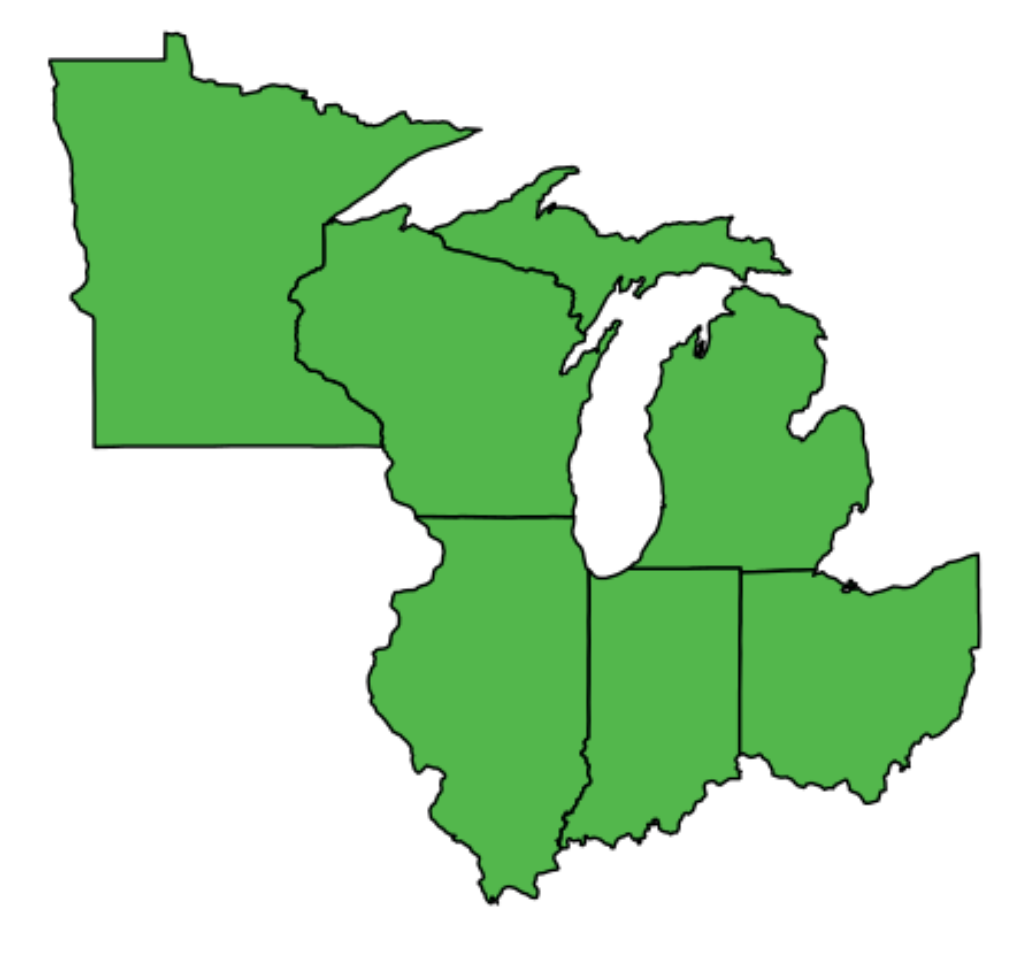
\includegraphics[valign = T,width=2cm]{/mnt/ceph/erichs/git/IMCI-covid-riskfinal/region_pngs/region5.png}\\
Region 6 & Housing Type, Population Density, Social Associations, Age over 65+, Voting & 426 & Food Insecurity, Diabetes, Voting & 427 &  & 422 & 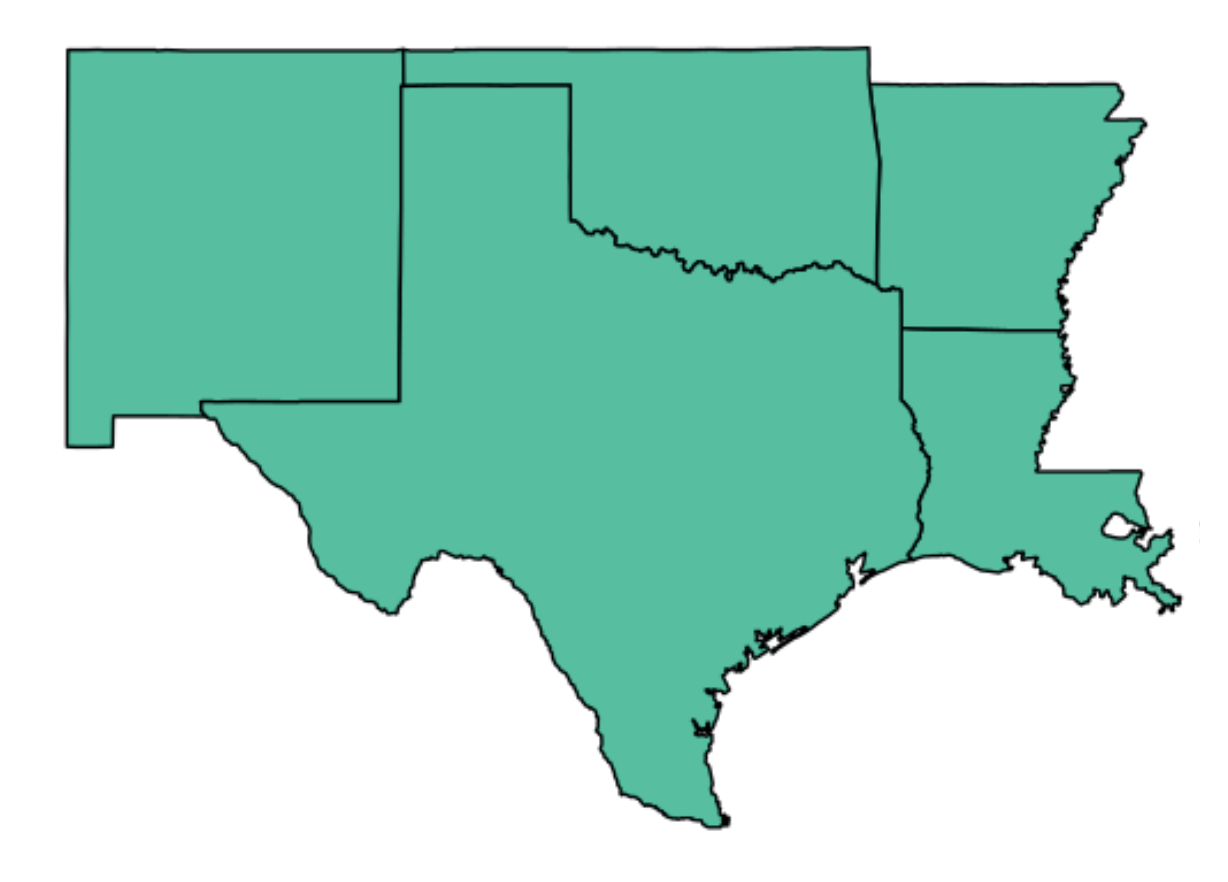
\includegraphics[valign = T,width=2cm]{/mnt/ceph/erichs/git/IMCI-covid-riskfinal/region_pngs/region6.png}\\
\addlinespace
Region 7 & Diabetes, Age over 65+, Vaccination Rate & 522 &  & 522 & Food Insecurity, Voting, Uninsured Adults & 522 & 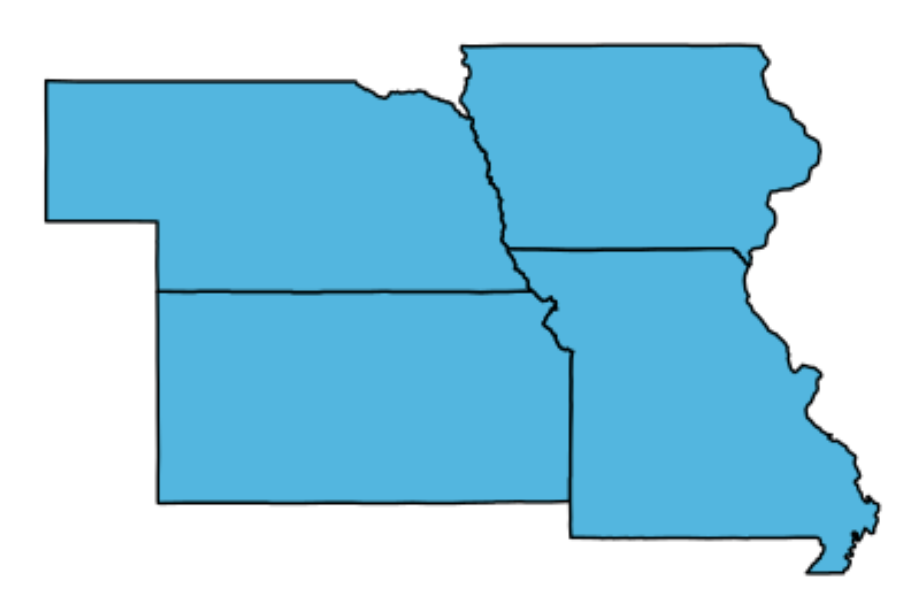
\includegraphics[valign = T,width=2cm]{/mnt/ceph/erichs/git/IMCI-covid-riskfinal/region_pngs/region7.png}\\
Region 8 &  & 382 &  & 382 & Household Composition, Broadband Access, Diabetes, Population Density, Age over 65+, Voting, Minority Status, Uninsured Adults & 382 & 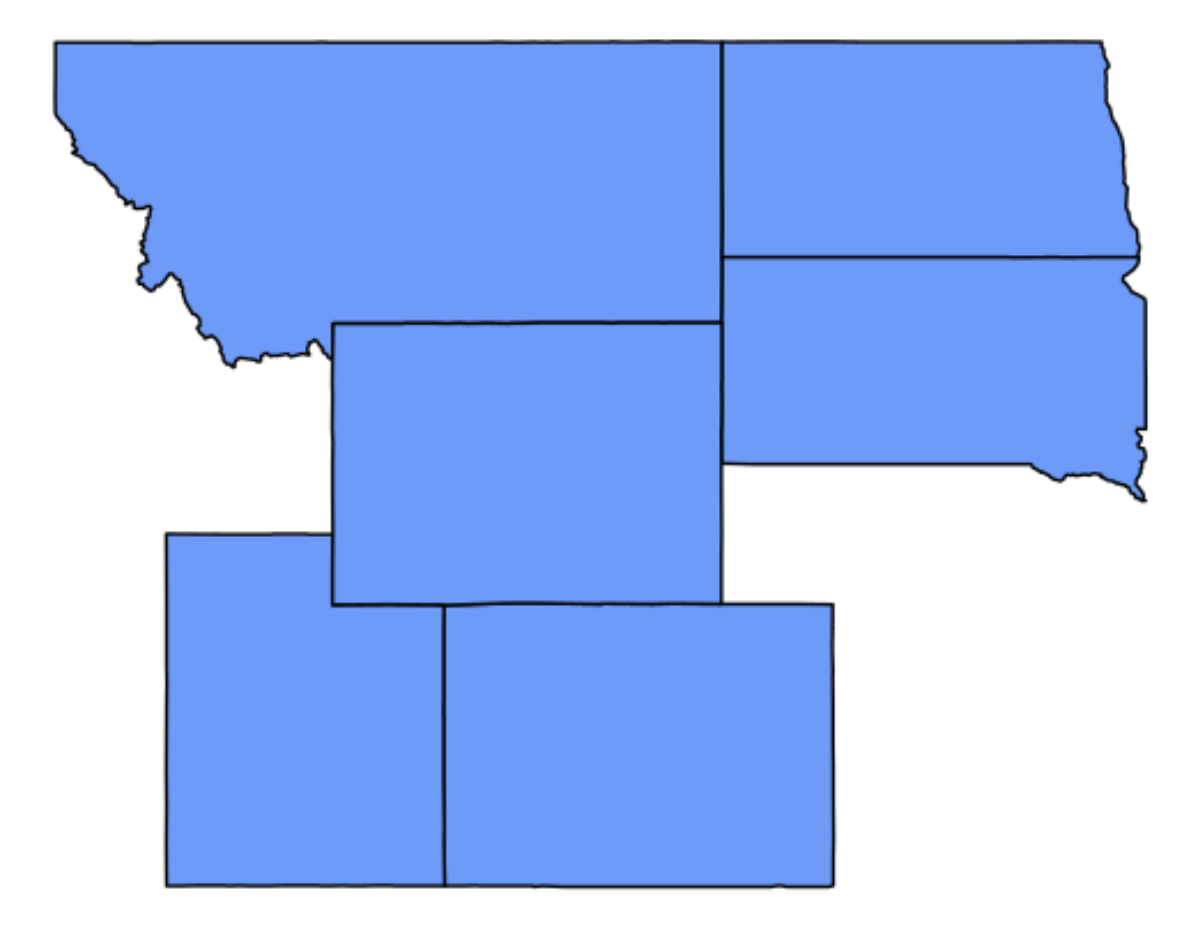
\includegraphics[valign = T,width=2cm]{/mnt/ceph/erichs/git/IMCI-covid-riskfinal/region_pngs/region8.png}\\
Region 9 & Vaccination Rate, Minority Status & 81 & Household Composition, Housing Type, Food Insecurity, Broadband Access, Diabetes, Obesity, Social Associations, Voting, Minority Status, Uninsured Adults & 81 & Obesity, Voting & 81 & 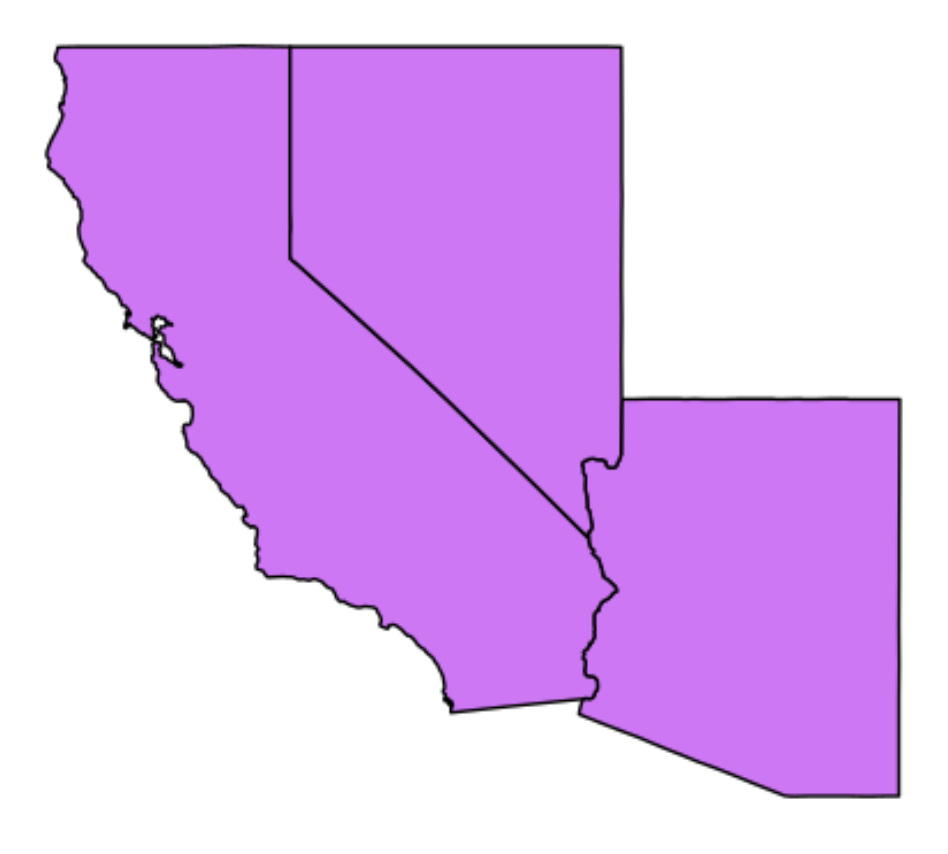
\includegraphics[valign = T,width=1.90cm]{/mnt/ceph/erichs/git/IMCI-covid-riskfinal/region_pngs/region9.png}\\
Region 10 & Age over 65+, Voting & 144 & Household Composition, Unemployment, Obesity, Age over 65+, Vaccination Rate & 144 & Diabetes, Minority Status & 142 & 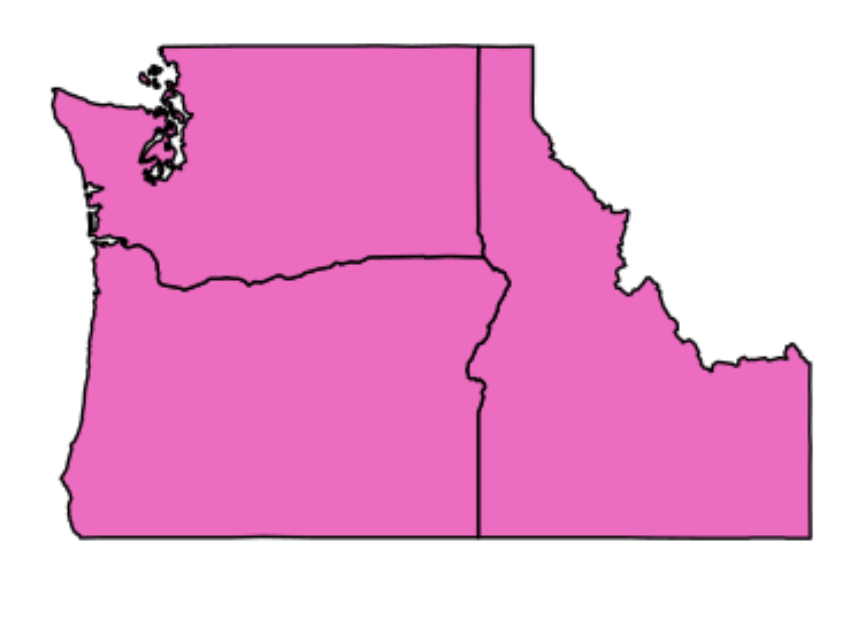
\includegraphics[valign = T,width=2cm]{/mnt/ceph/erichs/git/IMCI-covid-riskfinal/region_pngs/region10.png}\\
\bottomrule
\end{tabular}
\endgroup{}
\end{table}

\newpage

\hypertarget{part-4-spatial-autocorrelation-1}{%
\section{Part 4: Spatial
Autocorrelation}\label{part-4-spatial-autocorrelation-1}}

Morans I is a test of spatial autocorrelation.

\begin{displaymath}
I = \frac{n}{{{S_0}}}\frac{{\sum\limits_{i = 1}^n {\sum\limits_{j = 1}^n {{w_{ij}}\left( {{x_i} - \overline x } \right)\left( {{x_j} - \overline x } \right)} } }}{{\sum\limits_{i = 1}^n {{{\left( {{x_i} - \overline x } \right)}^2}} }}
\end{displaymath}

\begin{itemize}
\tightlist
\item
  N: The number of spatial units indexed by i and j
\item
  W: The sum of all wij
\item
  x: The variable of interest (in this instance, cumulative COVID cases,
  adjusted for population)
\item
  x: The mean of x
\item
  wij: A matrix of spatial weights
\end{itemize}

\newpage

\hypertarget{figure-s18-morans-i-results-united-states---alpha-wave-dependent-variable}{%
\subsection{Figure S18: Morans I results: United States - Alpha Wave,
Dependent
Variable}\label{figure-s18-morans-i-results-united-states---alpha-wave-dependent-variable}}

\includegraphics{test_0426_files/figure-latex/covidrisk_GWRF3b-1.pdf}

\newpage

\hypertarget{figure-s19-morans-i-results-united-states---alpha-wave-independent-variables}{%
\subsection{Figure S19: Morans I results: United States - Alpha Wave,
Independent
Variables}\label{figure-s19-morans-i-results-united-states---alpha-wave-independent-variables}}

\includegraphics{test_0426_files/figure-latex/covidrisk_moran_map1a-1.pdf}
\includegraphics{test_0426_files/figure-latex/covidrisk_moran_map1a-2.pdf}
\newpage
\includegraphics{test_0426_files/figure-latex/covidrisk_moran_map2a-1.pdf}
\includegraphics{test_0426_files/figure-latex/covidrisk_moran_map2a-2.pdf}
\newpage
\includegraphics{test_0426_files/figure-latex/covidrisk_moran_map3a-1.pdf}
\includegraphics{test_0426_files/figure-latex/covidrisk_moran_map3a-2.pdf}
\newpage
\includegraphics{test_0426_files/figure-latex/covidrisk_moran_map4a-1.pdf}
\includegraphics{test_0426_files/figure-latex/covidrisk_moran_map4a-2.pdf}
\newpage
\includegraphics{test_0426_files/figure-latex/covidrisk_moran_map5a-1.pdf}
\includegraphics{test_0426_files/figure-latex/covidrisk_moran_map5a-2.pdf}
\newpage
\includegraphics{test_0426_files/figure-latex/covidrisk_moran_map6a-1.pdf}
\includegraphics{test_0426_files/figure-latex/covidrisk_moran_map6a-2.pdf}
\newpage
\includegraphics{test_0426_files/figure-latex/covidrisk_moran_map7a-1.pdf}
\includegraphics{test_0426_files/figure-latex/covidrisk_moran_map7a-2.pdf}
\newpage
\includegraphics{test_0426_files/figure-latex/covidrisk_moran_map8a-1.pdf}
\newpage

\hypertarget{figure-s20-morans-i-results-united-states---delta-wave-dependent-variable}{%
\subsection{Figure S20: Morans I results: United States - Delta Wave,
Dependent
Variable}\label{figure-s20-morans-i-results-united-states---delta-wave-dependent-variable}}

\includegraphics{test_0426_files/figure-latex/covidrisk_GWRF4-1.pdf}

\hypertarget{figure-s21-morans-i-results-united-states---delta-wave-independent-variables}{%
\subsection{Figure S21: Morans I results: United States - Delta Wave,
Independent
Variables}\label{figure-s21-morans-i-results-united-states---delta-wave-independent-variables}}

\includegraphics{test_0426_files/figure-latex/covidrisk_moran_map1d-1.pdf}
\includegraphics{test_0426_files/figure-latex/covidrisk_moran_map1d-2.pdf}
\newpage
\includegraphics{test_0426_files/figure-latex/covidrisk_moran_map2d-1.pdf}
\includegraphics{test_0426_files/figure-latex/covidrisk_moran_map2d-2.pdf}
\newpage
\includegraphics{test_0426_files/figure-latex/covidrisk_moran_map3d-1.pdf}
\includegraphics{test_0426_files/figure-latex/covidrisk_moran_map3d-2.pdf}
\newpage
\includegraphics{test_0426_files/figure-latex/covidrisk_moran_map4d-1.pdf}
\includegraphics{test_0426_files/figure-latex/covidrisk_moran_map4d-2.pdf}
\newpage
\includegraphics{test_0426_files/figure-latex/covidrisk_moran_map5d-1.pdf}
\includegraphics{test_0426_files/figure-latex/covidrisk_moran_map5d-2.pdf}
\newpage
\includegraphics{test_0426_files/figure-latex/covidrisk_moran_map6d-1.pdf}
\includegraphics{test_0426_files/figure-latex/covidrisk_moran_map6d-2.pdf}
\newpage
\includegraphics{test_0426_files/figure-latex/covidrisk_moran_map7d-1.pdf}
\includegraphics{test_0426_files/figure-latex/covidrisk_moran_map7d-2.pdf}
\newpage
\includegraphics{test_0426_files/figure-latex/covidrisk_moran_map8d-1.pdf}
\newpage

\hypertarget{figure-s22-morans-i-results-united-states---omicron-wave-dependent-variable}{%
\subsection{Figure S22: Morans I results: United States - Omicron Wave,
Dependent
Variable}\label{figure-s22-morans-i-results-united-states---omicron-wave-dependent-variable}}

\includegraphics{test_0426_files/figure-latex/covidrisk_GWRF_omicron-1.pdf}

\hypertarget{figure-s23-morans-i-results-united-states---omicron-wave-independent-variables}{%
\subsection{Figure S23: Morans I results: United States - Omicron Wave,
Independent
Variables}\label{figure-s23-morans-i-results-united-states---omicron-wave-independent-variables}}

\includegraphics{test_0426_files/figure-latex/covidrisk_moran_map1o-1.pdf}
\includegraphics{test_0426_files/figure-latex/covidrisk_moran_map1o-2.pdf}
\newpage
\includegraphics{test_0426_files/figure-latex/covidrisk_moran_map2o-1.pdf}
\includegraphics{test_0426_files/figure-latex/covidrisk_moran_map2o-2.pdf}
\newpage
\includegraphics{test_0426_files/figure-latex/covidrisk_moran_map3o-1.pdf}
\includegraphics{test_0426_files/figure-latex/covidrisk_moran_map3o-2.pdf}
\newpage
\includegraphics{test_0426_files/figure-latex/covidrisk_moran_map4o-1.pdf}
\includegraphics{test_0426_files/figure-latex/covidrisk_moran_map4o-2.pdf}
\newpage
\includegraphics{test_0426_files/figure-latex/covidrisk_moran_map5o-1.pdf}
\includegraphics{test_0426_files/figure-latex/covidrisk_moran_map5o-2.pdf}
\newpage
\includegraphics{test_0426_files/figure-latex/covidrisk_moran_map6o-1.pdf}
\includegraphics{test_0426_files/figure-latex/covidrisk_moran_map6o-2.pdf}
\newpage
\includegraphics{test_0426_files/figure-latex/covidrisk_moran_map7o-1.pdf}
\includegraphics{test_0426_files/figure-latex/covidrisk_moran_map7o-2.pdf}
\newpage
\includegraphics{test_0426_files/figure-latex/covidrisk_moran_map8o-1.pdf}
\newpage

\end{document}
